% Schematic of the XSuM-MicroBooNE chain with the status of each step (2026-11-18).
% Compile: bash docs/technote/build.sh (standalone PDF, included by technote.tex). Update when a step changes status.
\documentclass[tikz,border=6pt]{standalone}
\usetikzlibrary{positioning,fit,arrows.meta,calc,backgrounds,shapes.symbols}
\usepackage[T1]{fontenc}
\usepackage{amsmath,amssymb}
\usepackage{helvet}\renewcommand{\familydefault}{\sfdefault}
\definecolor{ink}{HTML}{222222}
\definecolor{cdone}{HTML}{009E73}
\definecolor{cpart}{HTML}{E69F00}
\definecolor{cmiss}{HTML}{8C8C8C}
\definecolor{cext}{HTML}{0072B2}
\definecolor{chere}{HTML}{D55E00}
\tikzset{
  box/.style={draw=ink, line width=1pt, rounded corners=3pt, fill=white, align=left, inner sep=5pt, font=\scriptsize, text=ink, text width=36mm},
  done/.style={box, draw=cdone, line width=1.4pt, fill=cdone!8},
  part/.style={box, draw=cpart, line width=1.4pt, fill=cpart!10},
  miss/.style={box, draw=cmiss, dashed, fill=white, text=ink!75},
  ext/.style={box, draw=cext, line width=1.4pt, fill=cext!6},
  band/.style={font=\footnotesize\bfseries, text=ink!80, anchor=south west},
  lab/.style={font=\tiny, text=ink!70, align=center},
  arr/.style={-{Latex[length=2mm]}, line width=0.7pt, draw=ink},
  arrm/.style={arr, dashed, draw=ink!60},
  bg/.style={rounded corners=5pt, fill=ink!3, draw=ink!15, inner sep=5mm},
}
\begin{document}
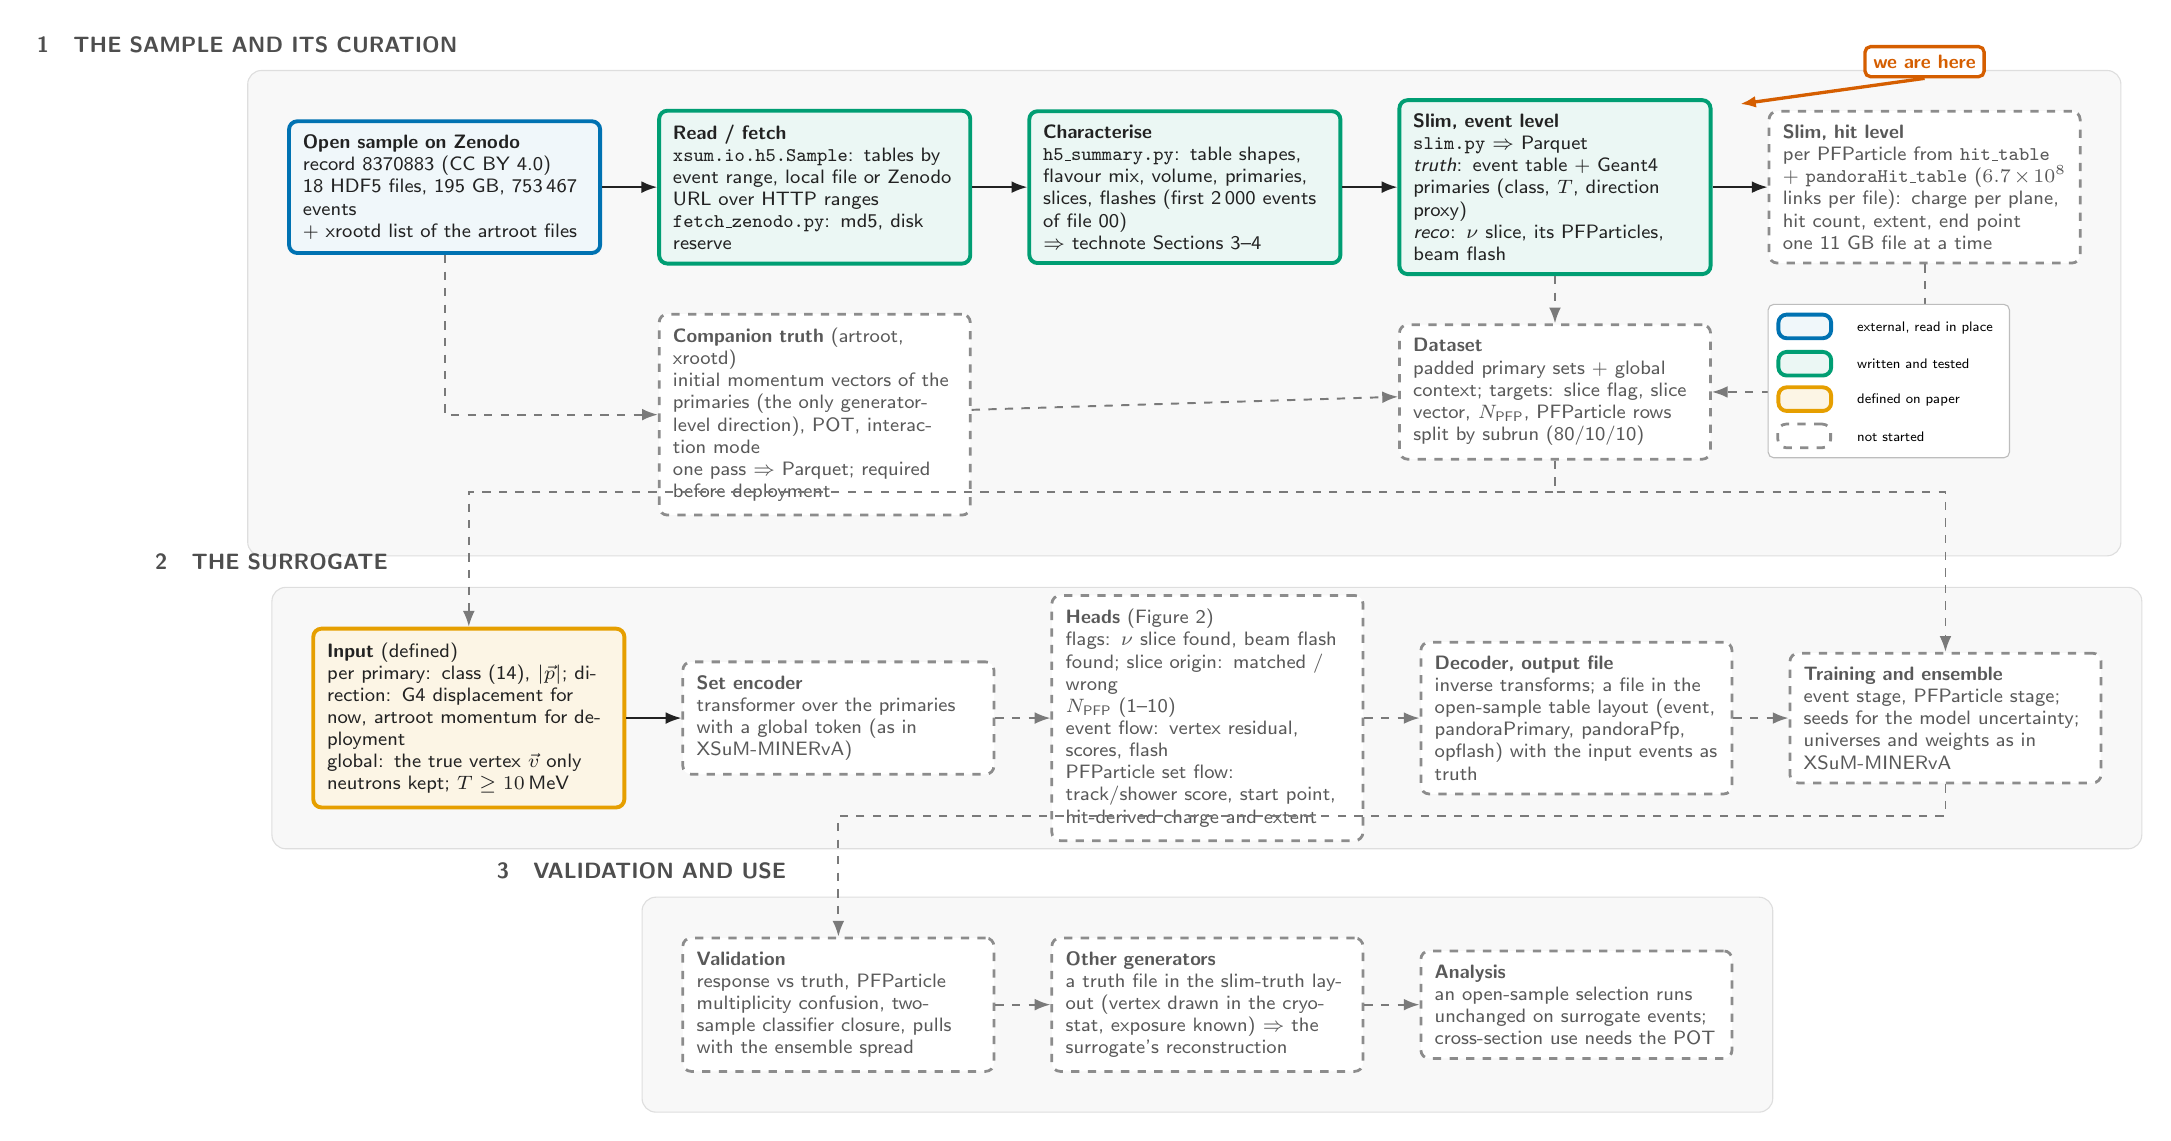
\begin{tikzpicture}[node distance=6mm and 7mm]

% ================= band 1: the sample and its curation =================
\node[ext] (zen) {\textbf{Open sample on Zenodo}\\ record 8370883 (CC BY 4.0)\\ 18 HDF5 files, 195 GB, 753\,467 events\\ + xrootd list of the artroot files};
\node[done, right=of zen] (read) {\textbf{Read / fetch}\\ \texttt{xsum.io.h5.Sample}: tables by event range, local file or Zenodo URL over HTTP ranges\\ \texttt{fetch\_zenodo.py}: md5, disk reserve};
\node[done, right=of read] (char) {\textbf{Characterise}\\ \texttt{h5\_summary.py}: table shapes, flavour mix, volume, primaries, slices, flashes (first 2\,000 events of file 00)\\ $\Rightarrow$ technote Sections 3--4};
\node[done, right=of char] (slim) {\textbf{Slim, event level}\\ \texttt{slim.py} $\Rightarrow$ Parquet\\ \emph{truth}: event table + Geant4 primaries (class, $T$, direction proxy)\\ \emph{reco}: $\nu$ slice, its PFParticles, beam flash};
\node[miss, right=of slim] (hits) {\textbf{Slim, hit level}\\ per PFParticle from \texttt{hit\_table} + \texttt{pandoraHit\_table} ($6.7\times10^8$ links per file): charge per plane, hit count, extent, end point\\ one 11 GB file at a time};

\node[miss, below=of read] (art) {\textbf{Companion truth} (artroot, xrootd)\\ initial momentum vectors of the primaries (the only generator-level direction), POT, interaction mode\\ one pass $\Rightarrow$ Parquet; required before deployment};
\node[miss, below=of slim] (ds) {\textbf{Dataset}\\ padded primary sets + global context; targets: slice flag, slice vector, $N_\text{PFP}$, PFParticle rows\\ split by subrun (80/10/10)};

\draw[arr] (zen) -- (read);
\draw[arr] (read) -- (char);
\draw[arr] (char) -- (slim);
\draw[arr] (slim) -- (hits);
\draw[arrm] (zen.south) |- (art.west);
\draw[arrm] (art) -- (ds);
\draw[arrm] (slim.south) -- (ds.north);
\draw[arrm] (hits.south) |- (ds.east);

% ================= band 2: the model =================
\node[part, below=14mm of art.south west, anchor=north west, xshift=-37mm-7mm] (inp) {\textbf{Input} (defined)\\ per primary: class (14), $|\vec p|$; direction: G4 displacement for now, artroot momentum for deployment\\ global: the true vertex $\vec v$ only\\ neutrons kept; $T \ge 10$\,MeV};
\node[miss, right=of inp] (enc) {\textbf{Set encoder}\\ transformer over the primaries with a global token (as in XSuM-MINERvA)};
\node[miss, right=of enc] (heads) {\textbf{Heads} (Figure 2)\\ flags: $\nu$ slice found, beam flash found; slice origin: matched / wrong\\ $N_\text{PFP}$ (1--10)\\ event flow: vertex residual, scores, flash\\ PFParticle set flow: track/shower score, start point, hit-derived charge and extent};
\node[miss, right=of heads] (dec) {\textbf{Decoder, output file}\\ inverse transforms; a file in the open-sample table layout (event, pandoraPrimary, pandoraPfp, opflash) with the input events as truth};
\node[miss, right=of dec] (train) {\textbf{Training and ensemble}\\ event stage, PFParticle stage; seeds for the model uncertainty; universes and weights as in XSuM-MINERvA};

\draw[arr] (inp) -- (enc);
\draw[arrm] (enc) -- (heads);
\draw[arrm] (heads) -- (dec);
\draw[arrm] (dec) -- (train);
\draw[arrm] (ds.south) -- ++(0,-4mm) -| (inp.north);
\draw[arrm] (ds.south) -- ++(0,-4mm) -| (train.north);

% ================= band 3: use =================
\node[miss, anchor=north west] (val) at ($(enc.north west |- heads.south)+(0,-12mm)$) {\textbf{Validation}\\ response vs truth, PFParticle multiplicity confusion, two-sample classifier closure, pulls with the ensemble spread};
\node[miss, right=of val] (gen) {\textbf{Other generators}\\ a truth file in the slim-truth layout (vertex drawn in the cryostat, exposure known) $\Rightarrow$ the surrogate's reconstruction};
\node[miss, right=of gen] (ana) {\textbf{Analysis}\\ an open-sample selection runs unchanged on surrogate events; cross-section use needs the POT};
\draw[arrm] (train.south) |- ++(-4mm,-4mm) -| (val.north);
\draw[arrm] (val) -- (gen);
\draw[arrm] (gen) -- (ana);

% ================= "we are here" =================
\node[draw=chere, line width=1.2pt, rounded corners=2pt, fill=white, font=\scriptsize\bfseries, text=chere, inner sep=3pt, above=4mm of hits.north] (here) {we are here};
\draw[-{Latex[length=2mm]}, line width=1.2pt, draw=chere] (here.south) -- ($(slim.north east)!0.5!(hits.north west)+(0,0)$);

% ================= band labels and backgrounds =================
\begin{scope}[on background layer]
  \node[bg, fit=(zen)(hits)(art)(ds)] (b1) {};
  \node[bg, fit=(inp)(train)] (b2) {};
  \node[bg, fit=(val)(ana)] (b3) {};
\end{scope}
\node[band, above=1mm of b1.north west] {1\quad THE SAMPLE AND ITS CURATION};
\node[band, above=1mm of b2.north west] {2\quad THE SURROGATE};
\node[band, above=1mm of b3.north west] {3\quad VALIDATION AND USE};

% ================= legend =================
\matrix[draw=ink!30, rounded corners=2pt, fill=white, inner sep=3pt, column sep=2mm, row sep=1mm, anchor=north west, font=\tiny] at ([yshift=-5mm]hits.south west) {
  \node[ext, text width=6mm, minimum height=3mm, inner sep=1pt]{}; & \node{external, read in place}; \\
  \node[done, text width=6mm, minimum height=3mm, inner sep=1pt]{}; & \node{written and tested}; \\
  \node[part, text width=6mm, minimum height=3mm, inner sep=1pt]{}; & \node{defined on paper}; \\
  \node[miss, text width=6mm, minimum height=3mm, inner sep=1pt]{}; & \node{not started}; \\
};
\end{tikzpicture}
\end{document}
